\section{Graph and network optimization}

\begin{figure}[H]
\centering
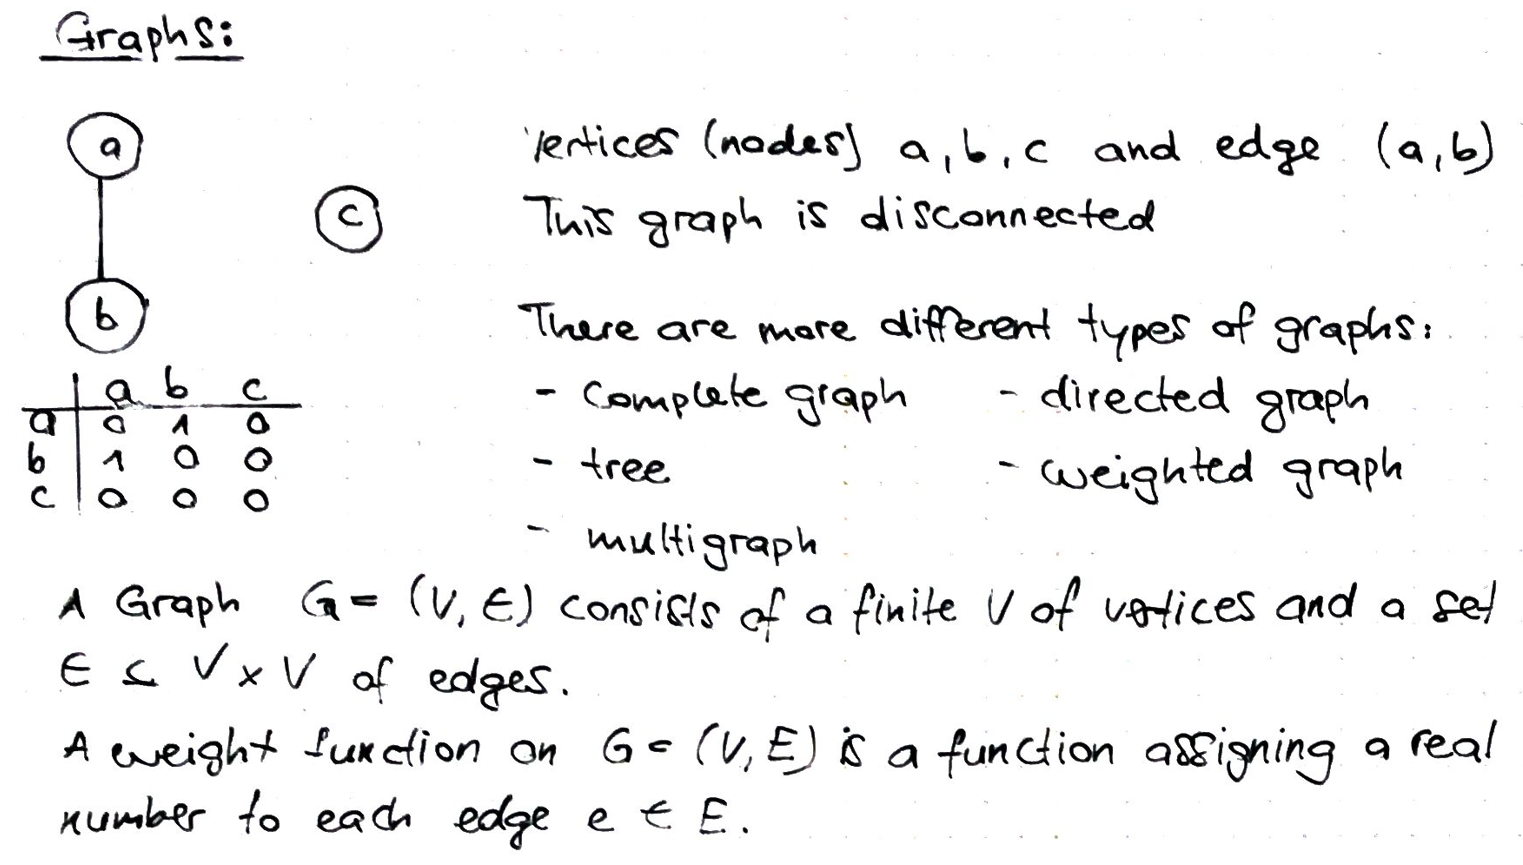
\includegraphics[width=1\textwidth]{figures/graphsIntroduction.png}
\caption{Introduction to Graphs}
\end{figure}

\begin{figure}[H]
\centering
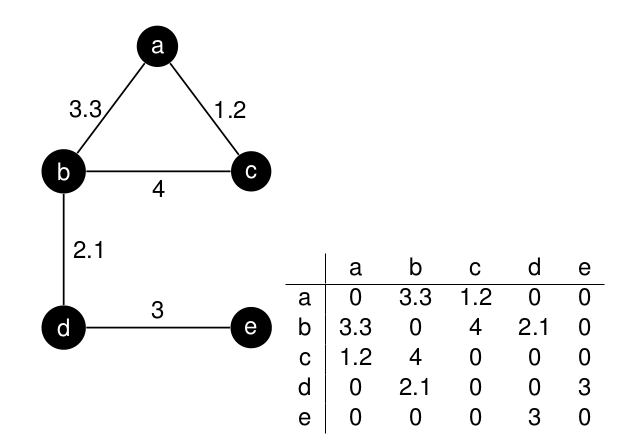
\includegraphics[width=0.5\textwidth]{figures/weightedAdjecency.png}
\caption{Example Graph with weight and Adjecency Matrix }
\end{figure}

\subsection{Depth-First Search (DFS)}

\begin{figure}[H]
\centering
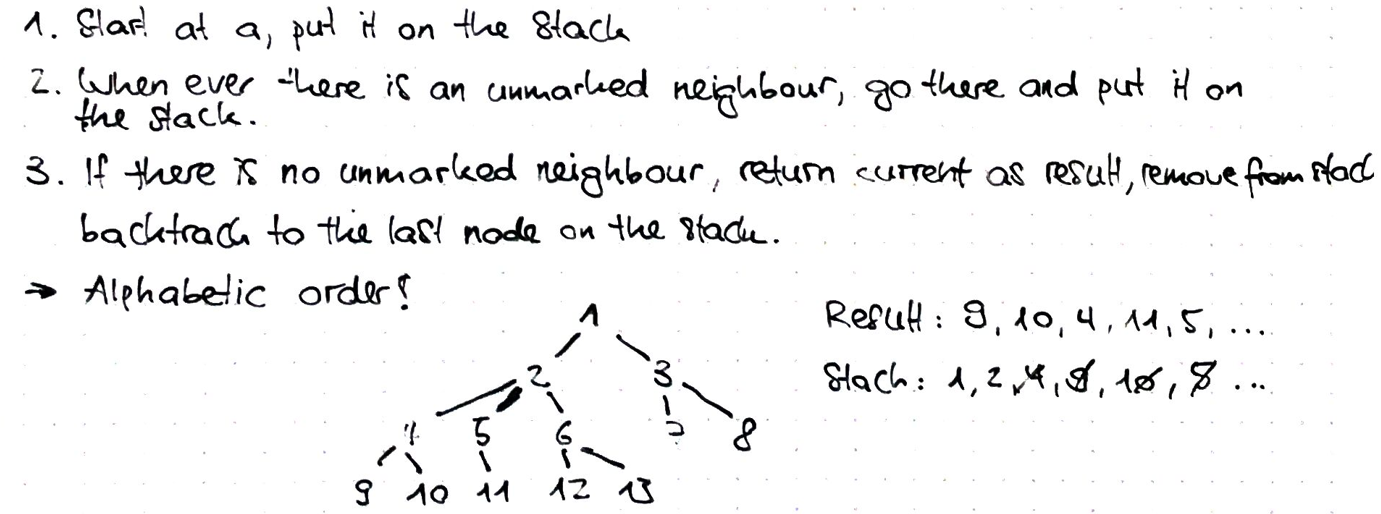
\includegraphics[width=1\textwidth]{figures/dfs.png}
\caption{Depth-First Search}
\end{figure}

\subsection{Breadth-First Search (BFS)}

\begin{figure}[H]
\centering
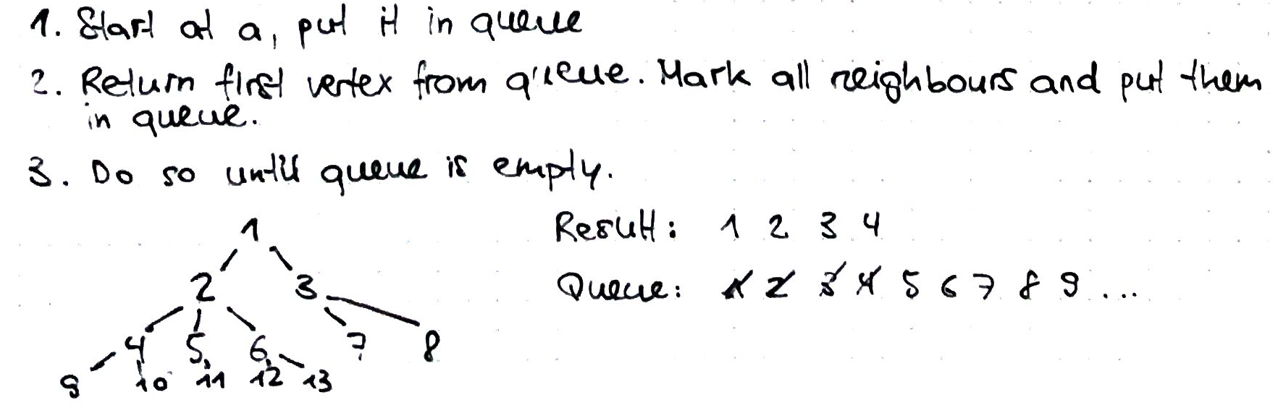
\includegraphics[width=1\textwidth]{figures/bfs.png}
\caption{Depth-First Search}
\end{figure}

\subsection{Spanning trees}

\begin{figure}[H]
\centering
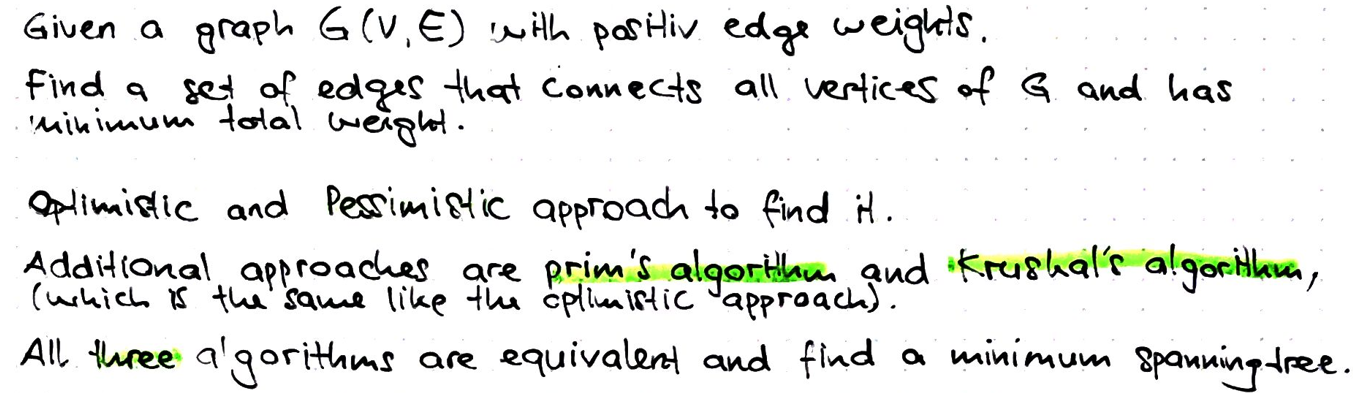
\includegraphics[width=1\textwidth]{figures/spanningtree.png}
\caption{Spanning trees}
\end{figure}

\subsubsection{Minimal weight Optimistic approach (And Kruskal’s algorithm)}

\textbf{The Kruskal algorithm is exactly the same approach like the optimistic approach.} \\
\textit{The Prim algorithm just differ a little bit since you have a starting node and then search within the connected edges.}

\begin{enumerate}
    \item Find the next edge with the lowest weight in the whole graph
    \item Check if the edge is redundant or not
    \item If the edge is not redundant, mark it as usable. If it is redundant, mark it as unusable
    \item Repeat until you have all edges checked
\end{enumerate}

\begin{figure}[H]
\centering
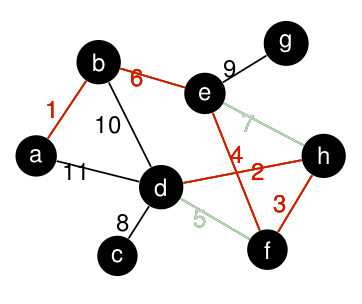
\includegraphics[width=0.3\textwidth]{figures/optimisticGraphAlg.png}
\caption{Minimal weight - Optimistic Approach}
\end{figure}

\subsubsection{Minimal weight Pessimistic approach}


\begin{enumerate}
    \item Find the next edge with the highest weight in the whole graph
    \item Check if you can remove the edge without splitting the graph into two graphs
    \item If you can remove the edge, mark it as unusable. If you can't remove the edge, mark it as usable
    \item Repeat until you have all edges checked
\end{enumerate}

\begin{figure}[H]
\centering
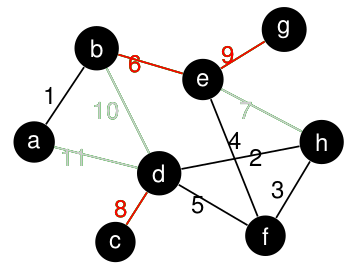
\includegraphics[width=0.3\textwidth]{figures/pessimisticGraphAlg.png}
\caption{Minimal weight - Pessimistic Approach}
\end{figure}

\clearpage
\subsubsection{Minimal weight Prim's algorithm}
Choose an arbitrary start vertex $v_0$ and set $M = \{v_0\}$.
Iteratively add to $M$ a vertex in $V \setminus M$ that can be reached the
cheapest from the current set $M$. Select the corresponding
edge. Continue until $M = V$ .

\begin{figure}[H]
\centering
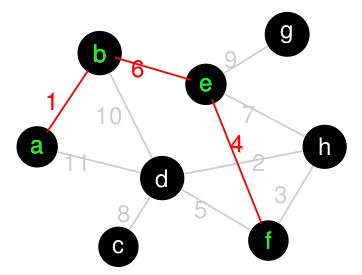
\includegraphics[width=0.3\textwidth]{figures/primsGraphAlg.png}
\caption{Minimal weight - Prim's Algorithm}
\end{figure}

\subsection{Shortes path problem}

\begin{figure}[H]
\centering
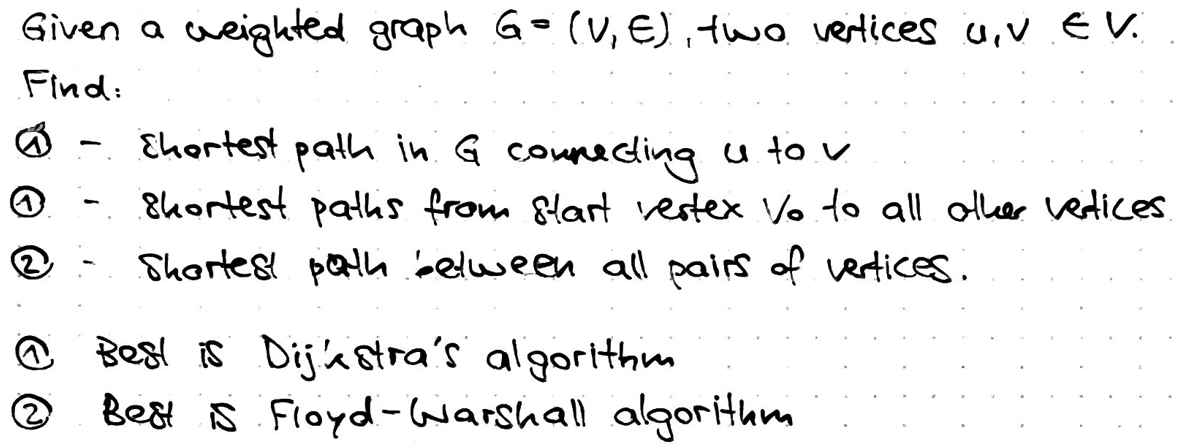
\includegraphics[width=1\textwidth]{figures/shortestPathProblem.png}
\caption{Spanning trees}
\end{figure}

\clearpage
\subsubsection{Dijkstra's algorithm}
Computes shortest paths from one vertex $v_0$ to all other vertices (i.e., a shortest-paths tree from $v_0$).
We iteratively compute the shortest distance $l(v)$ for the vertex
$v$ closest to $v_0$ that has not been reached yet, as follows:

\begin{enumerate}
    \item Set $V_0 = \{v_0\}, E_0 = \{\}$ and $I(v_0) = 0$
    \item Do the following $n-1$ times: \\
    $V_i = \{v_0, ..., v_i\}$ and $E_i = \{e_1, ..., e_i\}$ are the sets of vertices and edges already visited. For each edge $e = (u, v)$ with $u \in V_i$ and $v \in V \setminus V_i$, compute $l(u) + weight(e)$. Choose the edge minimizing this as $e_{i+1} = (u_{i+1}, v_{i+1})$. \\
    Set $V_{i+1} = V_i  \cup \{v_{i+1}\}, E_{i+1} = E_i \cup \{e_{i+1}\}$ and $l(v_{i+1}) = l(u_{i+1}) + weight(e_{i+1})$
\end{enumerate}

\begin{figure}[H]
\centering
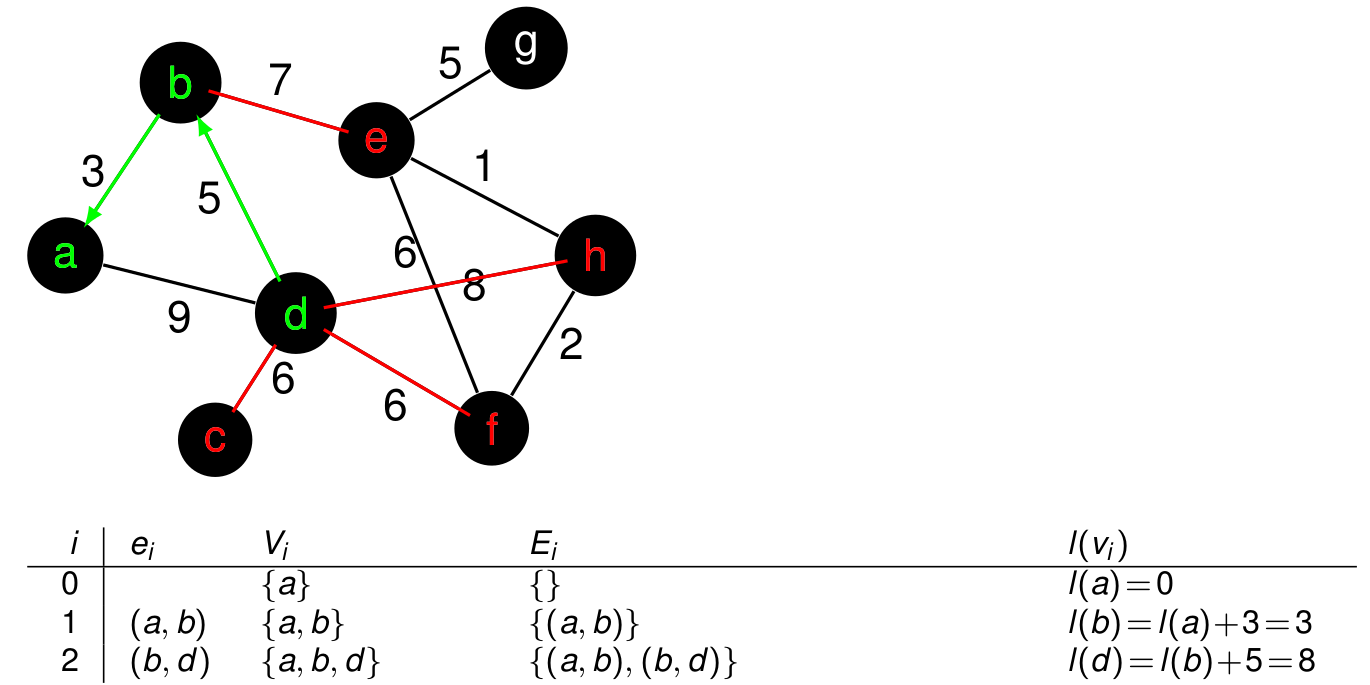
\includegraphics[width=0.8\textwidth]{figures/dijkstra.png}
\caption{Shortest Path - Dijkstra's Algorithm}
\end{figure}

\clearpage
\subsubsection{Floyd-Warshall algorithm}

The Floyd-Warshall algorithm solves the all-pairs shortest paths
problem. Unlike Dijkstra’s algorithm, it can also handle the case of
negative edge-weights.

\begin{enumerate}
    \item Initialization: \\
    $minPath(i, j, 0) =
  \begin{cases}
    w(v_i, v_j)       & \quad \text{if } (v_i, v_j) \in E\\
     \infty   & \quad \text{else}
  \end{cases}$
  \item For $k = 1,2,..., n$ compute: \\
  $minPath (i, j, k )$ for all $i$ und $j$ according iteration formula
\end{enumerate}

\begin{figure}[H]
\centering
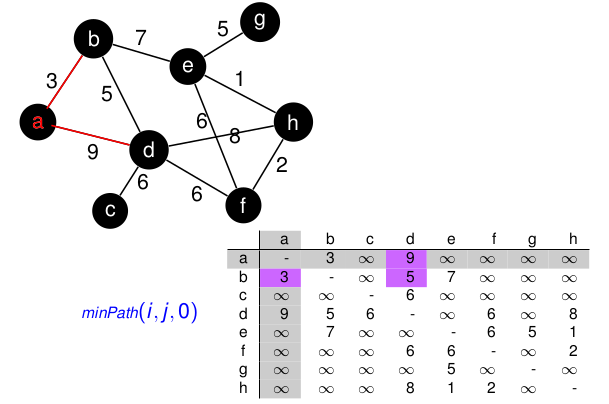
\includegraphics[width=0.6\textwidth]{figures/floyd1.png}
\caption{Shortest Path - Floyd-Warshall Matrix 1}
\end{figure}

\begin{itemize}
    \item Now I start with the first node $a$ and compare every other node if I can find a shorter path over $a$
    \item Starting this iteration with $b$, I check if I can find e.g. a shorter path from $b$ to $d$ over $a$.
    \item In this example, I see from $b$ to $d$ the weight is $5$. From $a$ to $b$ it is $3$, from $a$ to $d$ it is $9$, which would make a total of $12$. Since $12 \geq 5$, we leave $5$ and check the next node.
\end{itemize}

\begin{figure}[H]
\centering
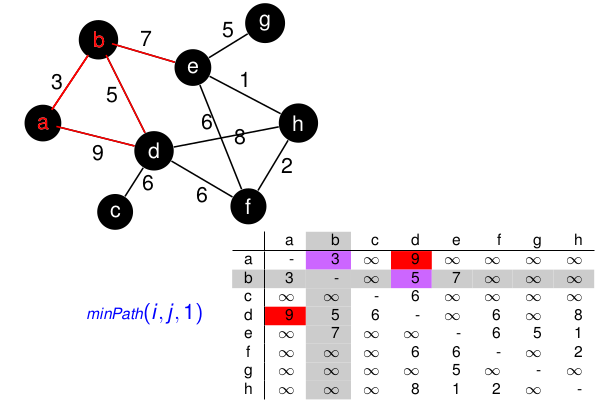
\includegraphics[width=0.6\textwidth]{figures/floyd2.png}
\caption{Shortest Path - Floyd-Warshall Matrix 2}
\end{figure}

\begin{itemize}
    \item After we have done this for every entry in the matrix compared to $a$, we start the next iteration step and comparing it with $b$
    \item In the next example, we found a improvement for the connection from $a$ to $d$. $a$ to $d$ has a weight of $9$, but if you go first from $a$ to $b$ with $3$, and then from $b$ to $d$ with $5$, you have a weight of $8$.
\end{itemize}

\begin{figure}[H]
\centering
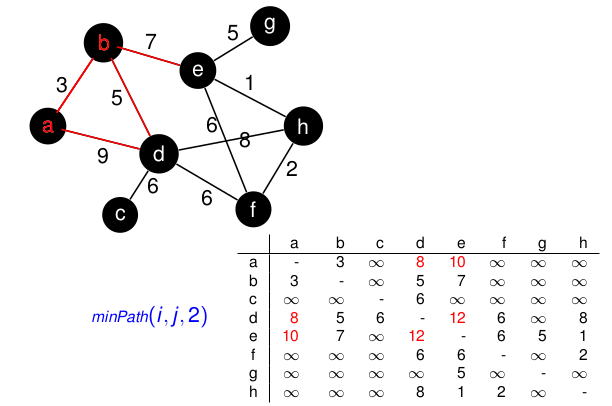
\includegraphics[width=0.6\textwidth]{figures/floyd3.png}
\caption{Shortest Path - Floyd-Warshall Matrix 3}
\end{figure}

\begin{itemize}
    \item After every iteration step, write the improvements directly into the matrix
    \item After comparing the entries in the matrix to every node, you should not have any $\infty$ anymore.
\end{itemize}

\clearpage
\subsection{Network flow}
\begin{figure}[H]
\centering
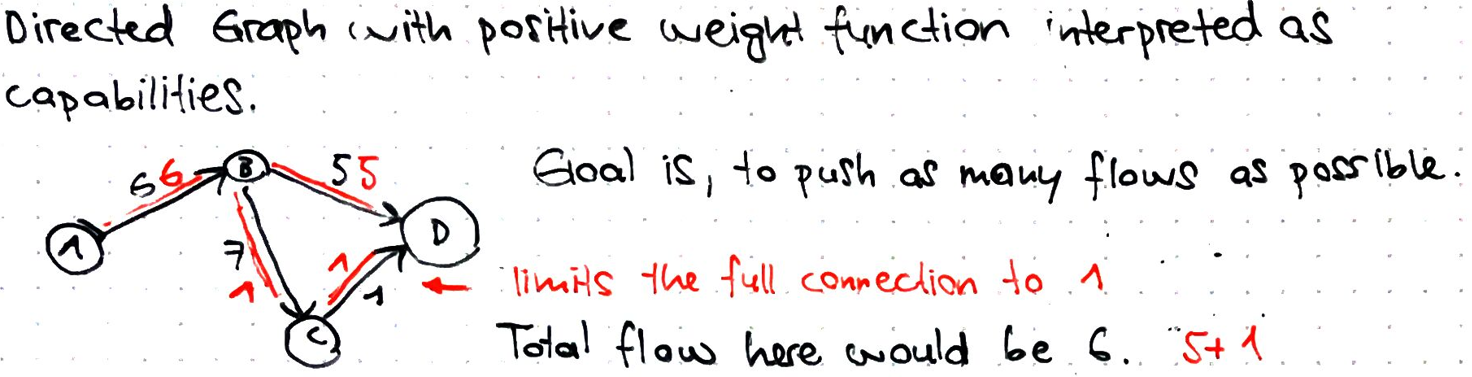
\includegraphics[width=0.8\textwidth]{figures/networkFlow.png}
\caption{Network Flow}
\end{figure}

\begin{tcolorbox}[colback=red!5!white,colframe=red!75!black]
An \textbf{st-network} $(G, w, s, t)$ is a weighted graph $G(V,E)$ with weight function $w$ and two distinguished vertices $s,t, \in V$, where $s$ is the source and $t$ is the target.
\end{tcolorbox}

\begin{tcolorbox}[colback=red!5!white,colframe=red!75!black]
A graph $G(V,E)$ is \textbf{bipartite} if its vertex set can be split in two parts $A$ and $B$ such that all edges have one vertex in $A$ and one in $B$.
\end{tcolorbox}

\subsubsection{Maximum Flow}

\begin{figure}[H]
\centering
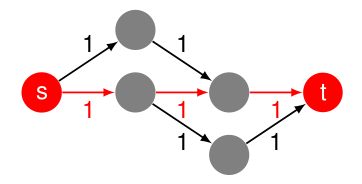
\includegraphics[width=0.3\textwidth]{figures/maximumFlow.png}
\caption{Maximum Network Flow Example}
\end{figure}

Finding the first best maximum network flow is not the best solution all the time. Sometimes, there are multiple paths and therefore you need to check more than one path. The Ford-Fulkerson algorithm checks already used paths for this.

\subsubsection{Ford-Fulkerson algorithm}
\begin{figure}[H]
\centering
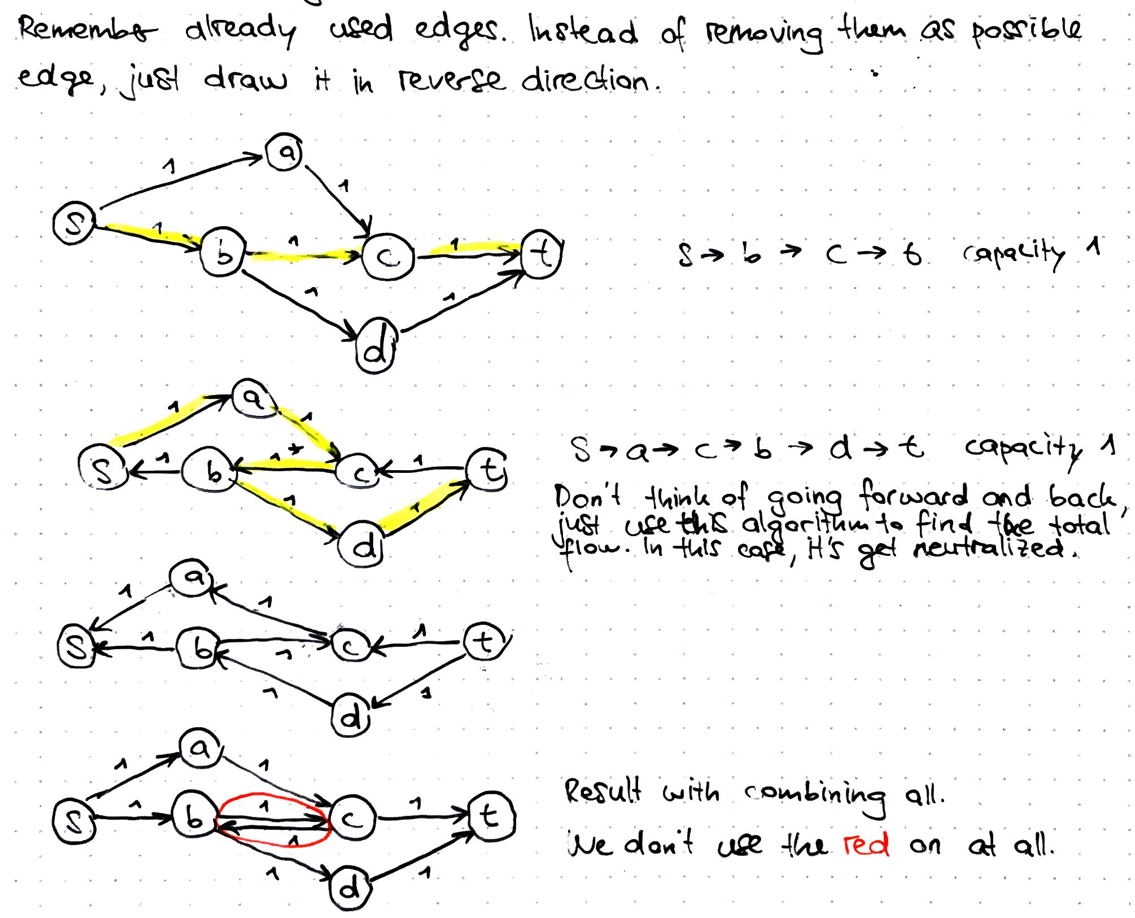
\includegraphics[width=0.9\textwidth]{figures/ford-fulkerson.png}
\caption{Ford Fulkerson algorithm}
\end{figure}

\subsubsection{Edmonds-Karp algorithm}
The Edmonds-Karp algorithm finds the path from $s$ to $t$ with the fewest number of edges. The algorithm is using Breadth-First Search for finding this.

\begin{figure}[H]
\centering
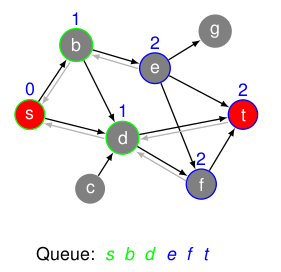
\includegraphics[width=0.3\textwidth]{figures/Edmonds-Karp.png}
\caption{Edmonds-Karp algorithm}
\end{figure}

\subsubsection{Distribution Problem}

\begin{figure}[H]
\centering
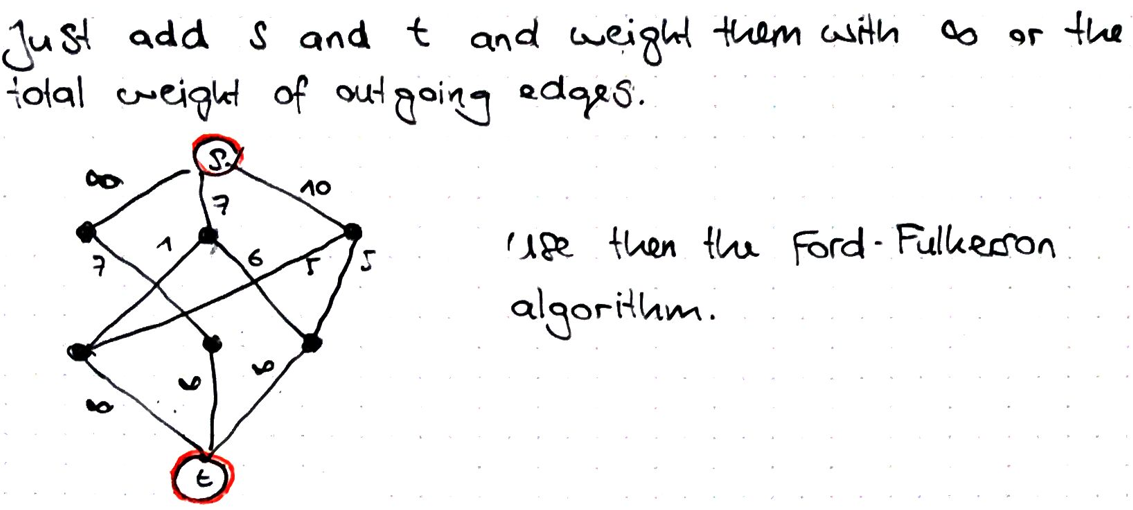
\includegraphics[width=0.9\textwidth]{figures/distributionProblem.png}
\caption{Network Flow - Distribution Problem}
\end{figure}

\subsubsection{Vertices with restrictions}

\begin{figure}[H]
\centering
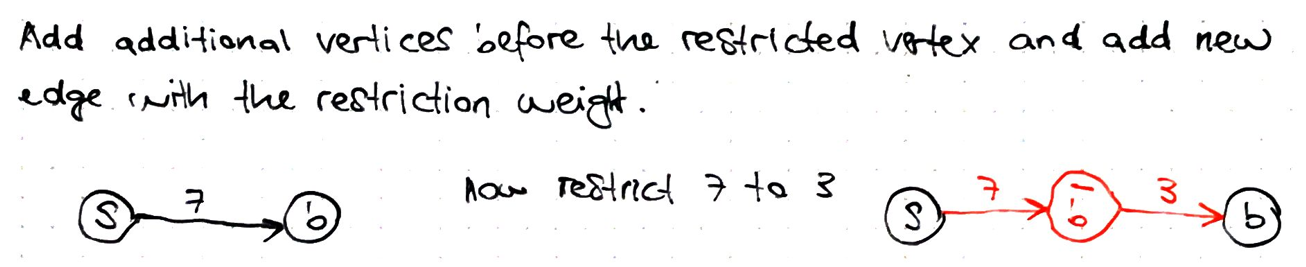
\includegraphics[width=0.9\textwidth]{figures/restrictionModelling.png}
\caption{Network Flow - Vertices with restrictions}
\end{figure}

\subsubsection{Bipartite Matching}

\begin{figure}[H]
\centering
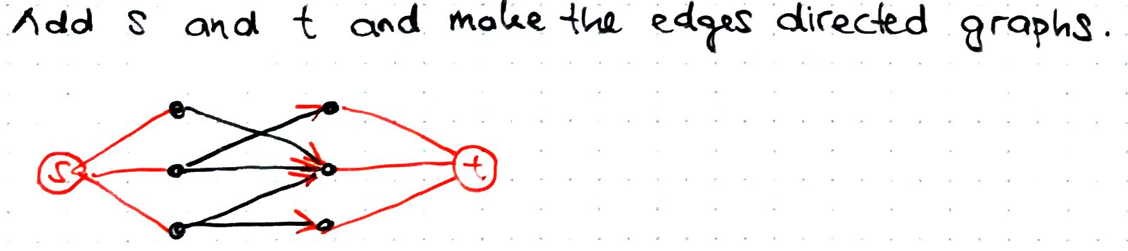
\includegraphics[width=0.9\textwidth]{figures/bipartiteMatching.png}
\caption{Network Flow - Bipartite Matching}
\end{figure}

\subsubsection{ST-Cut}

\begin{figure}[H]
\centering
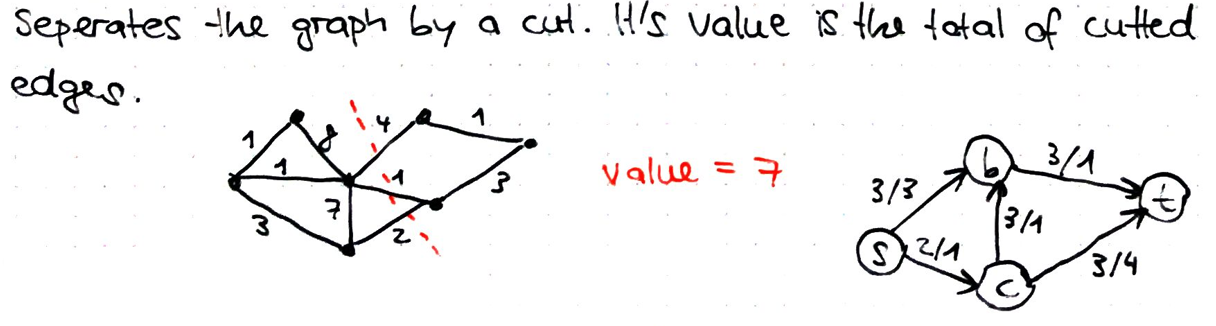
\includegraphics[width=0.9\textwidth]{figures/stCut.png}
\caption{Network Flow - ST-Cut}
\end{figure}

\begin{figure}[H]
\centering
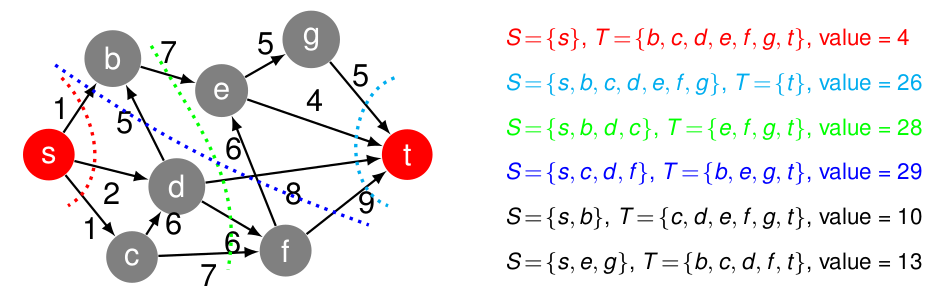
\includegraphics[width=0.6\textwidth]{figures/st-cut.png}
\caption{Network Flow - ST-Cut Example}
\end{figure}

\subsubsection{Min-Cost Max-Flow}

With the Ford-Fulkerson, there can be multiple solutions. You can now add costs to the edges and use this to find the best solution with the Ford-Fulkerson algorithm respecting the costs.

\begin{figure}[H]
\centering
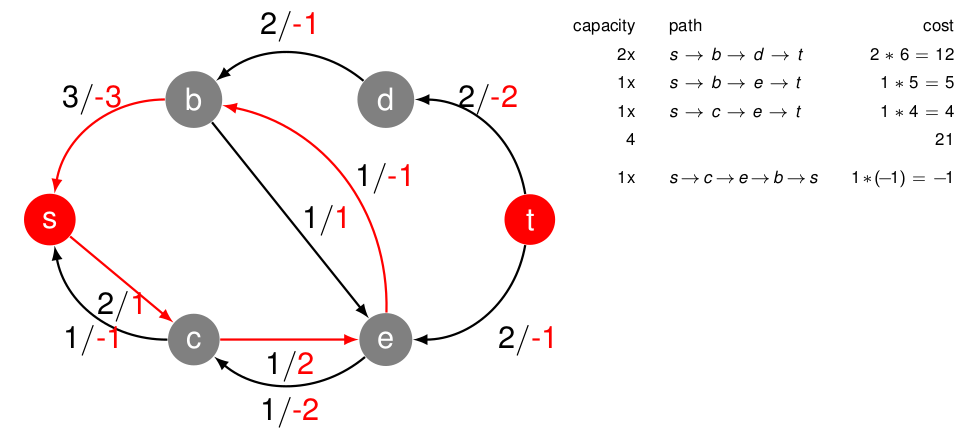
\includegraphics[width=0.6\textwidth]{figures/min-cost-max-flow.png}
\caption{Network Flow - Min-Cost Max-Flow}
\end{figure}

\clearpage